% ARRSI @ AACL-IJCNLP 2026 -- short paper (4 pages + references), *ACL format. Camera-ready.
\documentclass[11pt]{article}
\usepackage[final]{acl}
\usepackage{times}
\usepackage{latexsym}
\usepackage[T1]{fontenc}
\usepackage[utf8]{inputenc}
\usepackage{microtype}
\usepackage{inconsolata}
\usepackage{graphicx}
\usepackage{booktabs}
\usepackage{amsmath,amssymb,amsthm}
\newtheorem{proposition}{Proposition}
\newcommand{\OneModels}{118}
\newcommand{\OneItems}{2{,}985}
\newcommand{\OneSecondGap}{0.7}
\newcommand{\OneSecondCost}{0.7}
\newcommand{\OneSecondRemoved}{19}
\newcommand{\OneTopTwentyGap}{10.5}
\newcommand{\OneFreeCrownable}{118}
\newcommand{\OneFreeRatioMedian}{1.00}
\newcommand{\OneFreeRatioMax}{2.00}
\newcommand{\OneFreeRatioTopTwentyMax}{1.02}
\newcommand{\OneFreeRatioMin}{1.000}
\newcommand{\OneFreeKeepTopTwentyMin}{89.5}
\newcommand{\OneFreeAtKeepNinetyFive}{11}
\newcommand{\OneFreeAtKeepNinety}{19}
\newcommand{\OneFreeAtKeepEighty}{58}
\newcommand{\OneFreeAtKeepFifty}{117}
\newcommand{\OneStratCrownable}{118}
\newcommand{\OneStratRatioMedian}{1.39}
\newcommand{\OneStratRatioMax}{2.31}
\newcommand{\OneStratRatioTopTwentyMax}{2.24}
\newcommand{\OneStratRatioMin}{1.004}
\newcommand{\OneStratKeepTopTwentyMin}{81.8}
\newcommand{\OneStratAtKeepNinetyFive}{10}
\newcommand{\OneStratAtKeepNinety}{15}
\newcommand{\OneStratAtKeepEighty}{28}
\newcommand{\OneStratAtKeepFifty}{105}
\newcommand{\TwoModels}{188}
\newcommand{\TwoItems}{1{,}753}
\newcommand{\TwoSecondGap}{5.2}
\newcommand{\TwoSecondCost}{5.3}
\newcommand{\TwoSecondRemoved}{68}
\newcommand{\TwoTopTwentyGap}{13.8}
\newcommand{\TwoFreeCrownable}{188}
\newcommand{\TwoFreeRatioMedian}{1.00}
\newcommand{\TwoFreeRatioMax}{1.35}
\newcommand{\TwoFreeRatioTopTwentyMax}{1.03}
\newcommand{\TwoFreeRatioMin}{1.000}
\newcommand{\TwoFreeKeepTopTwentyMin}{86.2}
\newcommand{\TwoFreeAtKeepNinetyFive}{1}
\newcommand{\TwoFreeAtKeepNinety}{6}
\newcommand{\TwoFreeAtKeepEighty}{74}
\newcommand{\TwoFreeAtKeepFifty}{175}
\newcommand{\TwoStratCrownable}{188}
\newcommand{\TwoStratRatioMedian}{1.12}
\newcommand{\TwoStratRatioMax}{1.58}
\newcommand{\TwoStratRatioTopTwentyMax}{1.43}
\newcommand{\TwoStratRatioMin}{1.000}
\newcommand{\TwoStratKeepTopTwentyMin}{81.7}
\newcommand{\TwoStratAtKeepNinetyFive}{1}
\newcommand{\TwoStratAtKeepNinety}{3}
\newcommand{\TwoStratAtKeepEighty}{50}
\newcommand{\TwoStratAtKeepFifty}{171}
\newcommand{\OneKeepTwentyFive}{14}
\newcommand{\OneWinnersTwentyFive}{60}
\newcommand{\OneKeepFifty}{25}
\newcommand{\OneWinnersFifty}{33}
\newcommand{\OneKeepHundred}{35}
\newcommand{\OneWinnersHundred}{20}
\newcommand{\OneKeepTwoHundred}{48}
\newcommand{\OneWinnersTwoHundred}{12}
\newcommand{\OneKeepFiveHundred}{65}
\newcommand{\OneWinnersFiveHundred}{9}
\newcommand{\OneKeepThousand}{78}
\newcommand{\OneWinnersThousand}{6}
\newcommand{\OneNatWorstName}{donotanswer}
\newcommand{\OneNatWorstRank}{95}
\newcommand{\OneSectionWinnersDistinct}{3}
\newcommand{\TwoKeepTwentyFive}{41}
\newcommand{\TwoWinnersTwentyFive}{113}
\newcommand{\TwoKeepFifty}{66}
\newcommand{\TwoWinnersFifty}{64}
\newcommand{\TwoKeepHundred}{87}
\newcommand{\TwoWinnersHundred}{18}
\newcommand{\TwoKeepTwoHundred}{97}
\newcommand{\TwoWinnersTwoHundred}{5}
\newcommand{\TwoKeepFiveHundred}{100}
\newcommand{\TwoWinnersFiveHundred}{2}
\newcommand{\TwoKeepThousand}{100}
\newcommand{\TwoWinnersThousand}{1}
\newcommand{\TwoNatWorstName}{Safety}
\newcommand{\TwoNatWorstRank}{33}
\newcommand{\TwoSectionWinnersDistinct}{2}
\newcommand{\OneAttainable}{113}
\newcommand{\OneTrailing}{117}
\newcommand{\OneCertItems}{12}
\newcommand{\OneCertItemsSafe}{11}
\newcommand{\OneCertGap}{0.67}
\newcommand{\OneCertLP}{0.68}
\newcommand{\OneCertLPItems}{19}
\newcommand{\OnePlausHalfLo}{1}
\newcommand{\OnePlausHalfHi}{1}
\newcommand{\OnePlausOneLo}{3}
\newcommand{\OnePlausOneHi}{3}
\newcommand{\OnePlausTwoLo}{5}
\newcommand{\OnePlausTwoHi}{6}
\newcommand{\OnePlausFiveLo}{11}
\newcommand{\OnePlausFiveHi}{11}
\newcommand{\OnePlausTenLo}{19}
\newcommand{\OnePlausTenHi}{19}
\newcommand{\OneValHundred}{35}
\newcommand{\OneValHundredCertShare}{15}
\newcommand{\OneValHundredCert}{64}
\newcommand{\OneValHundredUncert}{30}
\newcommand{\OneValHundredCertShareOne}{57}
\newcommand{\OneValHundredCertOne}{45}
\newcommand{\OneValHundredUncertOne}{23}
\newcommand{\OneValHundredCertShareFive}{0}
\newcommand{\OneValHundredCertFive}{50}
\newcommand{\OneValHundredUncertFive}{35}
\newcommand{\OneValTwoHundred}{46}
\newcommand{\OneValTwoHundredCertShare}{8}
\newcommand{\OneValTwoHundredCert}{87}
\newcommand{\OneValTwoHundredUncert}{43}
\newcommand{\OneValTwoHundredCertLo}{81}
\newcommand{\OneValTwoHundredCertHi}{92}
\newcommand{\OneValTwoHundredUncertLo}{41}
\newcommand{\OneValTwoHundredUncertHi}{45}
\newcommand{\OneValTwoHundredCertCount}{151}
\newcommand{\OneValTwoHundredCertShareOne}{36}
\newcommand{\OneValTwoHundredCertOne}{66}
\newcommand{\OneValTwoHundredUncertOne}{35}
\newcommand{\OneValTwoHundredCertShareFive}{0}
\newcommand{\OneValTwoHundredCertFive}{--}
\newcommand{\OneValTwoHundredUncertFive}{46}
\newcommand{\OneValFiveHundred}{66}
\newcommand{\OneValFiveHundredCertShare}{3}
\newcommand{\OneValFiveHundredCert}{98}
\newcommand{\OneValFiveHundredUncert}{65}
\newcommand{\OneValFiveHundredCertShareOne}{27}
\newcommand{\OneValFiveHundredCertOne}{93}
\newcommand{\OneValFiveHundredUncertOne}{56}
\newcommand{\OneValFiveHundredCertShareFive}{0}
\newcommand{\OneValFiveHundredCertFive}{--}
\newcommand{\OneValFiveHundredUncertFive}{66}
\newcommand{\TwoCertItems}{43}
\newcommand{\TwoCertItemsSafe}{42}
\newcommand{\TwoCertGap}{5.22}
\newcommand{\TwoCertLP}{5.30}
\newcommand{\TwoCertLPItems}{68}
\newcommand{\TwoPlausHalfLo}{1}
\newcommand{\TwoPlausHalfHi}{1}
\newcommand{\TwoPlausOneLo}{1}
\newcommand{\TwoPlausOneHi}{1}
\newcommand{\TwoPlausTwoLo}{1}
\newcommand{\TwoPlausTwoHi}{1}
\newcommand{\TwoPlausFiveLo}{1}
\newcommand{\TwoPlausFiveHi}{1}
\newcommand{\TwoPlausTenLo}{6}
\newcommand{\TwoPlausTenHi}{6}
\newcommand{\TwoValHundred}{87}
\newcommand{\TwoValHundredCertShare}{76}
\newcommand{\TwoValHundredCert}{95}
\newcommand{\TwoValHundredUncert}{61}
\newcommand{\TwoValHundredCertShareOne}{92}
\newcommand{\TwoValHundredCertOne}{91}
\newcommand{\TwoValHundredUncertOne}{42}
\newcommand{\TwoValHundredCertShareFive}{36}
\newcommand{\TwoValHundredCertFive}{100}
\newcommand{\TwoValHundredUncertFive}{80}
\newcommand{\TwoValTwoHundred}{97}
\newcommand{\TwoValTwoHundredCertShare}{88}
\newcommand{\TwoValTwoHundredCert}{100}
\newcommand{\TwoValTwoHundredUncert}{75}
\newcommand{\TwoValTwoHundredCertLo}{99}
\newcommand{\TwoValTwoHundredCertHi}{100}
\newcommand{\TwoValTwoHundredUncertLo}{69}
\newcommand{\TwoValTwoHundredUncertHi}{80}
\newcommand{\TwoValTwoHundredCertCount}{1758}
\newcommand{\TwoValTwoHundredCertShareOne}{95}
\newcommand{\TwoValTwoHundredCertOne}{99}
\newcommand{\TwoValTwoHundredUncertOne}{55}
\newcommand{\TwoValTwoHundredCertShareFive}{45}
\newcommand{\TwoValTwoHundredCertFive}{100}
\newcommand{\TwoValTwoHundredUncertFive}{94}
\newcommand{\TwoValFiveHundred}{100}
\newcommand{\TwoValFiveHundredCertShare}{97}
\newcommand{\TwoValFiveHundredCert}{100}
\newcommand{\TwoValFiveHundredUncert}{97}
\newcommand{\TwoValFiveHundredCertShareOne}{99}
\newcommand{\TwoValFiveHundredCertOne}{100}
\newcommand{\TwoValFiveHundredUncertOne}{83}
\newcommand{\TwoValFiveHundredCertShareFive}{50}
\newcommand{\TwoValFiveHundredCertFive}{100}
\newcommand{\TwoValFiveHundredUncertFive}{100}


\title{Curated to Win: Certifying Reward-Model and Judge Selection\\Against Evaluation-Set Curation}

\author{Adrian Erlikhman \\
  Los Angeles Community College District \\
  \texttt{erlikhman.adrian@gmail.com}}

\begin{document}
\maketitle

\begin{abstract}
Automated research and self-improvement pipelines select a reward model or LLM judge by its accuracy on a validation set, and that set is often curated by the pipeline or its designers. We propose a \emph{curation certificate} for this selection: how much of the validation set could be removed without changing the winner. For weighted-accuracy benchmarks the certificate has a closed form. Measured in benchmark weight it is at least the gap between the top two models, and measured in items it is computed exactly by sorting per-item score differences. Linear programs over item weights, rounded to verified item subsets, show that the weight bound is tight near the top of RewardBench (\OneModels{} models, \OneItems{} items) and RewardBench~2 (\TwoModels{} models, \TwoItems{} items). RewardBench's leader is certified against the removal of any \OneCertItemsSafe{} items, and removing \OneCertItems{} particular items makes the runner-up the winner; RewardBench~2's leader is certified against any \TwoCertItemsSafe{}. At a curation budget of 1\% of benchmark weight, \OnePlausOneLo{} RewardBench models could win. The certificate also works on small validation sets: with 200 random items, selections whose top-two gap exceeds 2 points agree with the full-benchmark winner \OneValTwoHundredCert\% of the time, against \OneValTwoHundredUncert\% for the rest. We give a selection protocol that reports the certificate, or the set of possible winners when the certificate is below the curation budget.
\end{abstract}

\section{Introduction}

Systems that automate research or improve themselves need an evaluator: a reward model to optimise against, or an LLM judge that ranks candidate outputs \citep{lu2024aiscientist,zheng2023judging}. Evaluators are chosen by meta-evaluation, that is, by their agreement with human preference labels on a benchmark such as RewardBench \citep{lambert2024rewardbench,malik2025rewardbench2}. In an automated pipeline the items used for this choice are often selected by the pipeline itself: a filtered subset, a domain slice, or a small validation set. If the ranking of evaluators depends on which items are kept, whoever selects the items also selects the evaluator, which is reward hacking one level above the reward \citep{gao2022overoptimization}. A selection should therefore come with a statement of how much curation it survives.

Leaderboards are known to be sensitive to benchmark choice, answer format and private testing \citep{dehghani2021lottery,alzahrani2024targets,singh2025illusion,zhang2024tradeoffs}, and to targeted edits of individual items \citep{dubrovsky2025selective}. \citet{gordienko2026rig} count the \emph{datasets} a developer must train on to top a multi-task leaderboard and show that the problem is NP-hard under mean win rate, and \citet{oyarhoseini2026perturbation} show with influence approximations that sub-1\% edits to pairwise matches can change the leader of a Bradley--Terry arena. Both describe how rankings can be attacked. We instead give the party selecting an evaluator a certificate it can compute and report, for the weighted-accuracy scores used in reward-model and judge meta-evaluation. Our contributions are:
\begin{itemize}\setlength\itemsep{0pt}
\item Two curation certificates for the winner of a weighted-accuracy benchmark: a lower bound in benchmark weight and an exact value in items (Props.~\ref{prop:floor}--\ref{prop:items}).
\item Evidence from linear programs on RewardBench and RewardBench~2 that the weight bound is tight near the top of both leaderboards.
\item Two applications: sets of possible winners at a given curation budget, and certificates computed on small validation sets, which separate reliable selections from unreliable ones.
\end{itemize}

\section{Setup}

A benchmark has items $i=1,\dots,N$ with official weights $w^0_i\ge 0$, $\sum_i w^0_i=1$. Model $m$ has per-item score $r_{mi}\in[0,1]$ and official score $S_m=\sum_i w^0_i r_{mi}$. A \emph{curation} keeps a set $K$ with kept share $f=\sum_{i\in K}w^0_i$ and rescores every model on it, $S^K_m=\sum_{i\in K}w^0_i r_{mi}/f$. We call $1-f$ the \emph{removed share}; $K$ \emph{crowns} $m$ if $S^K_m>S^K_k$ for every $k\neq m$.

\paragraph{Data.} RewardBench v1 publishes per-item results for \OneModels{} models on \OneItems{} preference pairs in 23 subsets \citep{lambert2024rewardbench}. We rebuild each official score from them: a section score is the count-weighted mean of its subset accuracies, with \texttt{math-prm} upweighted as in the released code, and the overall score is the mean of the four section scores. For four models, from the leader to a 0.5B chat model, our subset accuracies match RewardBench's published values exactly. Result files are aligned by position; a text check found no misaligned items. RewardBench~2 \citep{malik2025rewardbench2} publishes results by item id. We use the \TwoModels{} models with results on all \TwoItems{} items of its five accuracy subsets, scored as the mean of subset accuracies, and exclude the Ties subset, which uses a different metric.

\section{Curation Certificates}

Let $a$ be the winner and, for each challenger $c$, let $g_c=S_a-S_c>0$ and $d^c_i=w^0_i(r_{ai}-r_{ci})$.

\begin{proposition}\label{prop:floor}
Every $K$ with $S^K_c\ge S^K_a$ removes a share of at least $g_c$. Hence the winner is certified against any curation that removes a share below $g^\star=\min_c g_c$, the gap to the runner-up.
\end{proposition}
\begin{proof}
$f\,(S^K_a-S^K_c)=\sum_{i\in K}d^c_i=g_c-\sum_{i\notin K}d^c_i\ge g_c-(1-f)$, since $d^c_i\le w^0_i$; this is positive whenever $1-f<g_c$.
\end{proof}

\begin{proposition}\label{prop:items}
Sort $d^c_{(1)}\ge d^c_{(2)}\ge\cdots$ and let $k_c=\min\{k:\sum_{j\le k}d^c_{(j)}>g_c\}$. Removing a set $R$ makes $c$ overtake $a$ if and only if $\sum_{i\in R}d^c_i>g_c$, so no removal of fewer than $k_c$ items does, and removing the top $k_c$ items does. The winner is therefore certified against the removal of any $k^\star-1$ items, where $k^\star=\min_c k_c$, and this is exact.
\end{proposition}
\begin{proof}
From the identity above, $S^K_c>S^K_a$ iff $\sum_{i\notin K}d^c_i>g_c$. Any $k$ removed items contribute at most $\sum_{j\le k}d^c_{(j)}$.
\end{proof}
Both certificates need only the per-item score table: $g^\star$ is read off the leaderboard, and $k^\star$ costs one sort per challenger. Prop.~\ref{prop:floor} is a lower bound, since removing items that favour the winner over one challenger can let a third model overtake both. To test how tight it is, we compute for each model $m$ the largest kept share $f$ at which some curation crowns it. For fixed $f$, relaxing the subset to weights $w$ gives a linear program:
\begin{align*}
\max_{w,t}\; t \;\;\text{s.t.}\;\; &\textstyle\sum_i w_i (r_{mi}-r_{ki})\ge t \;\;\forall k\neq m,\\
&0\le w_i\le w^0_i/f,\quad \textstyle\sum_i w_i=1,
\end{align*}
and $m$ is crownable at $f$ if $t^*>0$. We scan $f$ downward from 1 and bisect, round each solution to an item subset by keeping the items at or near their upper bound, and accept it only if $m$ is still strictly first after rescoring, so every reported cost belongs to a verified subset. A \emph{section-preserving} variant also fixes each section's total weight, so the curated set keeps the benchmark's composition; since any verified section-preserving subset is also valid without the constraint, we report the unconstrained cost as the smaller of the two. For ordinal aggregates such as mean win rate, the analogous selection problem is NP-hard \citep{gordienko2026rig}; for weighted accuracy each check is a linear program.

\paragraph{Possible winners.} At curation budget $\delta$, let $P(\delta)$ be the set of models that some curation removing at most $\delta$ can crown. By Prop.~\ref{prop:floor}, $P(\delta)\subseteq\{m: S_a-S_m\le\delta\}$, and every model with a verified LP cost at most $\delta$ is in $P(\delta)$, which brackets its size.

\section{Results}

\begin{figure*}[t]
\centering
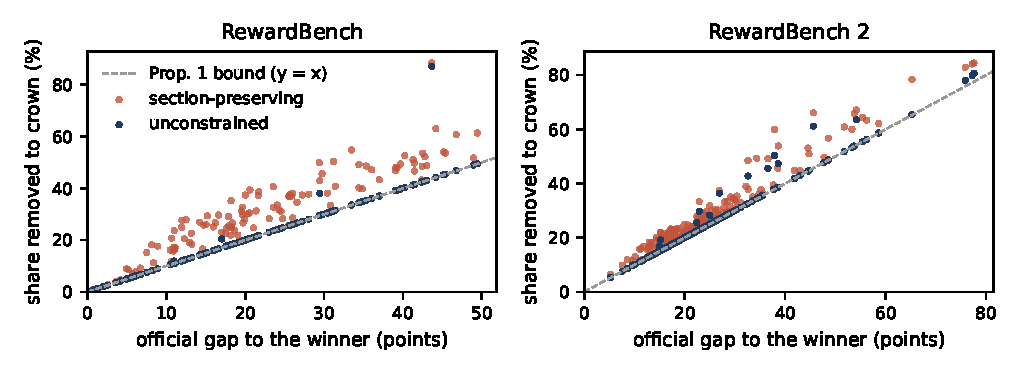
\includegraphics[width=0.85\textwidth]{fig_cost}
\caption{Share of the benchmark removed to crown each model, against its official gap to the winner. Every point lies on or above the dashed line $y=x$, the bound of Prop.~\ref{prop:floor}. Unconstrained curation reaches the bound for nearly every model; keeping each section's share costs more, at most \OneStratRatioMax{} times the gap.}
\label{fig:cost}
\end{figure*}

\paragraph{Certificates of the two leaders.} RewardBench's winner leads by $g^\star=\OneCertGap$ points, so it survives any curation removing less than \OneCertGap\% of benchmark weight; the smallest verified crowning curation removes \OneCertLP\%, so the certificate is tight to within 0.01 points. In items, the winner survives the removal of any \OneCertItemsSafe{} items, and removing \OneCertItems{} particular items makes the runner-up the new winner, which we verified by rescoring. (The LP, which minimises weight rather than count, used \OneCertLPItems{} items.) RewardBench~2's winner leads by \TwoCertGap{} points, needs \TwoCertLP\% removed, and is certified against any \TwoCertItemsSafe{} items.

\paragraph{The weight bound is tight near the top.} Every model on both benchmarks can be crowned. The ratio of removed share to gap has a median of \OneFreeRatioMedian{} on RewardBench and at most \OneFreeRatioTopTwentyMax{} in its top 20 (Figure~\ref{fig:cost}); the largest ratio over all models is \OneFreeRatioMax{}. Every top-20 model can be crowned while keeping at least \OneFreeKeepTopTwentyMin\% of the benchmark. On RewardBench~2 the median is \TwoFreeRatioMedian{} and the maximum \TwoFreeRatioMax{}. A curator who also keeps each section's share, leaving no trace in the per-section breakdown, pays a median of \OneStratRatioMedian{} times the gap on RewardBench and \TwoStratRatioMedian{} on RewardBench~2.

\begin{table}[t]
\centering\small
\begin{tabular}{lccccc}
\toprule
Budget $\delta$ & 0.5\% & 1\% & 2\% & 5\% & 10\%\\
\midrule
RewardBench & 1 & 3 & 5--6 & 11 & 19\\
RewardBench~2 & 1 & 1 & 1 & 1 & 6\\
\bottomrule
\end{tabular}

\caption{Number of possible winners $|P(\delta)|$ at curation budget $\delta$ (share of benchmark weight). A range gives the lower bound from verified LP curations and the upper bound from Prop.~\ref{prop:floor}.}
\label{tab:plausible}
\end{table}

\paragraph{Possible winners.} Because the bound is tight, the bracket on $P(\delta)$ is narrow (Table~\ref{tab:plausible}). On RewardBench a pipeline that may have curated 1\% of the benchmark can only say that one of \OnePlausOneLo{} models is best, and at 5\% one of \OnePlausFiveLo{}. RewardBench~2's winner is unique up to a 5\% budget.

\begin{table}[t]
\centering\small
\resizebox{\columnwidth}{!}{\begin{tabular}{rcccccc}
\toprule
& \multicolumn{3}{c}{RewardBench} & \multicolumn{3}{c}{RewardBench~2}\\
\cmidrule(lr){2-4}\cmidrule(lr){5-7}
$n$ & all & cert. & not & all & cert. & not\\
\midrule
100 & 35 & 64 {\scriptsize(15)} & 30 & 87 & 95 {\scriptsize(76)} & 61\\
200 & 46 & 87 {\scriptsize(8)} & 43 & 97 & 100 {\scriptsize(88)} & 75\\
500 & 66 & 98 {\scriptsize(3)} & 65 & 100 & 100 {\scriptsize(97)} & 97\\
\bottomrule
\end{tabular}
}
\caption{Validation sets of $n$ items drawn in proportion to official weight (2{,}000 draws). ``All'': share of selections equal to the full-benchmark winner. ``Cert.'': the same among selections whose top-two gap on the validation set exceeds 2 points (share of draws in brackets). ``Not'': among the rest.}
\label{tab:valcert}
\end{table}

\paragraph{Certificates on small validation sets.} A pipeline usually scores candidates on a small validation set, where the certificate is the top-two gap on that set. Table~\ref{tab:valcert} draws such sets at random, so that a set's mean is an unbiased estimate of the official score. On RewardBench, a 100-item set selects the full-benchmark winner in \OneValHundred\% of draws; with 200 items, the \OneValTwoHundredCertShare\% of selections certified at 2 points agree with it \OneValTwoHundredCert\% of the time, against \OneValTwoHundredUncert\% for the rest. On RewardBench~2, whose winner leads by \TwoCertGap{} points, most selections are certified and nearly all are correct. The certificate thus separates selections a pipeline can trust from those it should not, using only the validation scores.

\section{A Selection Protocol}

For an automated pipeline that selects an evaluator: (i) fix and hash the validation items before any candidate is scored, and log every filter applied to them; (ii) set a curation budget $\delta$ for how much of the set could have been dropped or filtered; (iii) report the certificates $g^\star$ and $k^\star$ with the selection, and accept the winner only if $g^\star>\delta$; (iv) otherwise report the possible-winner set, bracketed as above, rather than a single winner. The certificates cost one pass over the score table, so the protocol adds no model calls.

\section*{Limitations}
We study one curation operation, removing items, on two reward-model benchmarks. Reweighting the kept items, paraphrasing them or changing the prompt format would give a curator more freedom, so the certificates hold only against removal. The item certificate is exact; the LP costs are achievable but may not be minimal. The validation-set experiment draws random sets, not adversarial ones, and uses one threshold (2 points). We do not claim that any published result was curated. RewardBench~2's Ties subset is excluded, so its scores differ slightly from the official ones.

\section*{Reporting and Reproducibility}
All results come from public per-item result files (\texttt{allenai/reward-bench-results}, \texttt{allenai/reward-bench-2-results}). All analysis ran on one laptop CPU with SciPy's HiGHS solver; each full LP sweep takes one to two hours, the certificates seconds, and no models were run. One failed run is worth reporting: the first section-preserving search began its bisection at a very small kept share, where rounding can empty a section, and wrongly reported the leader as not crownable; the corrected search scans from $f=1$ downward. Code and derived data are at \url{https://github.com/adrian-erlikhman/curated-to-win}.

\section*{Use of AI Assistants}
An AI assistant (Claude, Anthropic) helped write the analysis code and draft the text. The author chose the study, checked the proofs and the results, and takes responsibility for the content.

\bibliography{references}

\end{document}
